% ; whizzy paragraph -pdf xpdf -latex ./whizzypdfptex.sh
% ; whizzy-paragraph "^\\\\begin{frame}"
% latex beamer presentation.
% platex, latex-beamer でコンパイルすることを想定。 

% Tokyo Debian Meeting resources
% Copyright (C) 2009 Junichi Uekawa
% Copyright (C) 2009 Nobuhiro Iwamatsu

% This program is free software; you can redistribute it and/or modify
% it under the terms of the GNU General Public License as published by
% the Free Software Foundation; either version 2 of the License, or
% (at your option) any later version.

% This program is distributed in the hope that it will be useful,
% but WITHOUT ANY WARRANTY; without even the implied warreanty of
% MERCHANTABILITY or FITNESS FOR A PARTICULAR PURPOSE.  See the
% GNU General Public License for more details.

% You should have received a copy of the GNU General Public License
% along with this program; if not, write to the Free Software
% Foundation, Inc., 51 Franklin St, Fifth Floor, Boston, MA  02110-1301 USA

\documentclass[cjk,dvipdfmx,12pt]{beamer}
\usetheme{Tokyo}
\usepackage{monthlypresentation}
\usepackage{listings}

\usepackage{ulem}

% preview (shell-command (concat "evince " (replace-regexp-in-string "tex$" "pdf"(buffer-file-name)) "&")) 
% presentation (shell-command (concat "xpdf -fullscreen " (replace-regexp-in-string "tex$" "pdf"(buffer-file-name)) "&"))
% presentation (shell-command (concat "evince " (replace-regexp-in-string "tex$" "pdf"(buffer-file-name)) "&"))

% http://www.naney.org/diki/dk/hyperref.html
% 日本語EUC系環境の時
\AtBeginDvi{\special{pdf:tounicode EUC-UCS2}}
% シフトJIS系環境の時
% \AtBeginDvi{\special{pdf:tounicode 90ms-RKSJ-UCS2}}


\title{GPG 秘密鍵取り扱い方法の提案}
\subtitle{}
\author{吉田 晋}
\date{2014年6月14日}
\logo{
\includegraphics[width=8cm]{image200607/openlogo-light.eps}}

\begin{document}
\lstset{ %
  backgroundcolor=\color{dancerlightblue},
  language=sh
}

\frame{\titlepage{}}

\begin{frame}{自己紹介}{}
  \begin{itemize}
  \item[名前] 吉田 晋 (wbcchsyn)

    ハンドルネームに特に由来は無い

    昔生成したランダム文字列

    (日本語では、「うぶちん」と名乗ったりもします。)

    どんなサービスであれ、

    このアカウントの人がいたら、多分私。
  \item[仕事] IT 系の会社でサーバーサイドの事を広く浅く

    UI は苦手
  \item[言語] いろんな言語を趣味として学ぶのが好き

    今年はアセンブリを覚えようと計画中
  \item[GPG] 4096R/DD08DFA8
  \end{itemize}
\end{frame}

\begin{frame}{自己紹介}{}
  セキュリティに関する座右の銘
  \vspace{1cm}

  \begin{itemize}
  \item 独自実装はするな、必ず穴がある
  \item 専門家の意見に従え
  \end{itemize}
  \vspace{1cm}

  セキュリティの専門家ではありません
\end{frame}

\begin{frame}{はじめに}{}
  みなさん、GPG のキーサインしていますか?
\end{frame}

\begin{frame}{はじめに}{}
  私は、
  \vspace{1cm}

  「大統一 Debian 勉強会 2013」
  \vspace{1cm}

  で初めてキーサインパーティーに参加しました
\end{frame}

\begin{frame}{はじめに}{}
  キーサインを行っている人は、
  \vspace{1cm}

  その秘密鍵はどうやって保管していますか?
\end{frame}

\begin{frame}{はじめに}{}
  再発行出来るとはいえ、秘密鍵が無くなると色々と不便
  \vspace{1cm}

  \begin{itemize}
  \item その秘密鍵で暗号化したファイルを

    復号化出来なくなる
  \item 再度、他の人に署名してもらう必要あり

    (貰ったキーサインは資産)
  \end{itemize}
  \vspace{1cm}

  記録メディアの破損等に備え、秘密鍵のバックアップは必要
\end{frame}

\begin{frame}{はじめに}{}
  一方、いつでも Revoke できるとはいえ、
  \vspace{1cm}

  最低限のマナーとして盗難や盗聴に気をつける必要も有り
  \vspace{1cm}

  管理強化の為には、鍵のバックアップは少ない方が有利
\end{frame}

\begin{frame}{はじめに}{}
  データの冗長性と管理強化、一見矛盾する要件ですが
  \vspace{1cm}

  みなさん、どうしてますか?
\end{frame}

\begin{frame}{はじめに}{}
  \begin{center}
    \textcolor{blue}{\LARGE {\bf {\it Fin}}}
  \end{center}
\end{frame}

\begin{frame}{はじめに}{}
  \begin{center}
    \sout{\textcolor{blue}{\LARGE {\bf {\it Fin}}}}

    {\LARGE ウソ}
  \end{center}
\end{frame}

\begin{frame}{はじめに}{}
  私は、今の所
  \vspace{1cm}

  「データは 3 カ所以上で保存しない」
  \vspace{1cm}

  という自分ルールで妥協中
\end{frame}

\begin{frame}{はじめに}{}
  今回は、この運用方法を変えたいと思って

  鍵管理ツールのプロトタイプを作ってみました。
  \vspace{1cm}

  ただ、自分はセキュリティについて詳しく無いので

  何かフィードバックがあれば、お願いします
  \vspace{1cm}

  「危険だからそんなツール使うな」

  って言う意見でも O.K. です
\end{frame}

\begin{frame}{アイディア}{}
  アイディアのベースは RAID3 (RAID5)
\end{frame}

\begin{frame}{アイディア}{}
  RAID3 ディスクアレイの特徴
  \begin{itemize}
  \item ディスク 1 本破損してもデータ復元可能
  \item ディスク 1 本盗難にあっても盗難者はデータ復旧不可能
  \end{itemize}
\end{frame}

\begin{frame}{アイディア}{}
  同じ要領でファイルを分散、保存

  メディアが 1 個破損してもデータ復旧可能

  メディアが 1 個盗まれても、しばらく大丈夫
  \vspace{1cm}

  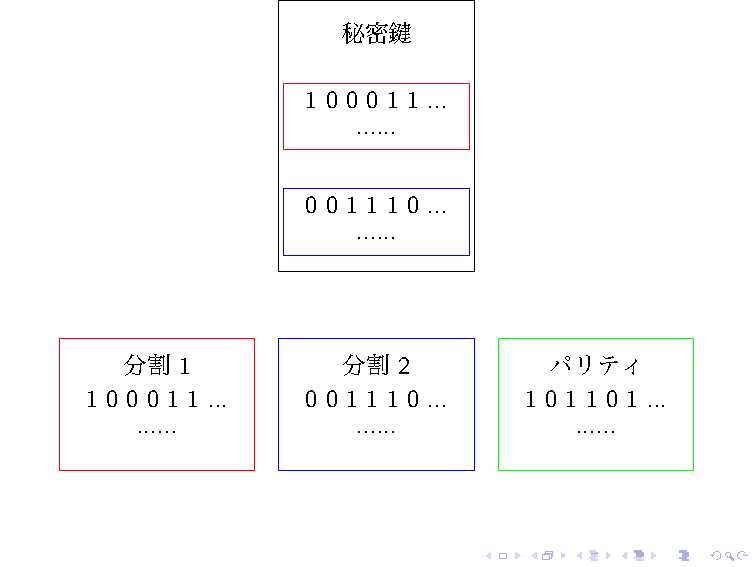
\includegraphics[width=8cm]{image201406/split_image.pdf}
\end{frame}

\begin{frame}{アイディア}{}
  例えば、3 個のファイルを

  PC、USB メモリ、DVD@金庫

  の 3 カ所に保存
  \vspace{1cm}

  普段は PC と USB メモリからデータを復旧させて使う

  (毎回、データ復旧、使い終わったら削除)

  なんて使い方を考え中
\end{frame}

\begin{frame}{アイディア}{}
  USB メモリに鍵情報を保存するのは少し怖いが、

  4096 bit 長の鍵ならば、ファイルが 1 個盗まれたとしても

  まだ 2048 bit 残っている
  \vspace{1cm}

  現役で 2048 bit 長の鍵を使っている人が居る事を思えば

  まだ大丈夫かなと。。。
\end{frame}

\begin{frame}{アイディア}{}
  ちなみに、分散するファイル数とパリティの数を

  それぞれ 2 倍にすると (4分割 + パリティ 2 個)
  \vspace{1cm}

  ファイル 1 個あたりの情報量 減

  メディア破損時の冗長性 増
  \vspace{1cm}

  ちゃんと、盗難時のリスク管理と冗長性の向上を両立出来てます。
\end{frame}

\begin{frame}{アイディア}{}
  完全な形のファイルを、どこにも保存する必要が無い事も

  個人的にはポイント高!
\end{frame}

\begin{frame}{実装紹介}{}
  ファイルを分割、分割したファイルを結合する

  プロトタイプを実装
  \vspace{1cm}

  \url{https://github.com/wbcchsyn/dVault_prototype.git}
  \vspace{1cm}

  dVault (distribute vault) と命名
\end{frame}

\begin{frame}{実装紹介}{}
  {\LARGE \textcolor{red}{注意}}

  これはプロトタイプです。

  絶対に、自分の秘密鍵で実験しないでください!
  \vspace{1cm}

  例えば、
  \begin{itemize}
  \item ファイルのアクセス権とか考えていません
  \item 問答無用で既存のファイルを上書きします

    失敗して、既存のファイルを壊すかも
  \end{itemize}
\end{frame}

\begin{frame}{実装紹介}{}
  分割したファイルの形式

  \begin{enumerate}
  \item ファイルの先頭に json 形式でメタデータを記載
  \item メタデータの後に空行を 1 行挟む
  \item その後、各ファイルにデータを保存
  \end{enumerate}
\end{frame}

\begin{frame}{実装紹介}{}
  現状では、下記の 3 個のメタデータを定義

  (このデータが無いと、復旧できない!)

  \begin{itemize}
  \item united\_length

    元ファイルのファイルサイズ
  \item split\_count

    ファイルを何分割したか

    (最低2, パリティの数は含まれません)
  \item index

    分割したフィアルの何個目か

    0 スタート

    index {\textgreater}= split\_count の場合、パリティである事を示す
  \end{itemize}
\end{frame}

\begin{frame}[containsverbatim]{使用方法}
  origin というファイルを split0, split1, parity の 3 個に分割

  \begin{commandline}
$ dvault split -u origin -s split0 -s split1 -s parity
  \end{commandline}
  \vspace{1cm}

  split0, parity の 2 個のファイルから origin を復旧

  \begin{commandline}
$ dvault unite -u origin -s split0 -s parity
  \end{commandline}
\end{frame}

\begin{frame}{実演}{}
  {\LARGE 実演}
\end{frame}

\begin{frame}[containsverbatim]{実演}{}
  中身が\verb|abcedf\n|の 7 byte のファイルを 3 個に分割してみる
\end{frame}

\begin{frame}[containsverbatim]{実演}{}
  準備

  \begin{commandline}
$ ls -l

total 4
-rw-r--r-- 1 wbcchsyn wbcchsyn 7 Jun 14 07:08 origin


$ cat origin

abcdef
  \end{commandline}
\end{frame}


\begin{frame}[containsverbatim]{実演}{}
  分割

  split0 には、ヘッダと origin の偶数バイト目が記載される

  \begin{commandline}
$ dvault split -u origin -s split0 -s split1 -s parity

$ cat split0

{"index": 0, "united_length": 7, "split_count": 2}

ace
  \end{commandline}
\end{frame}

\begin{frame}[containsverbatim]{実演}{}
  split0 と parity から origin を復活させる

  \begin{commandline}
$ rm origin split1

$ ls -l

total 8
-rw-r--r-- 1 wbcchsyn wbcchsyn 56 Jun 14 07:15 parity
-rw-r--r-- 1 wbcchsyn wbcchsyn 56 Jun 14 07:15 split0

$ dvault unite -u origin -s split0 -s parity

$ ls -l

total 12
-rw-r--r-- 1 wbcchsyn wbcchsyn  7 Jun 14 07:20 origin
-rw-r--r-- 1 wbcchsyn wbcchsyn 56 Jun 14 07:15 parity
-rw-r--r-- 1 wbcchsyn wbcchsyn 56 Jun 14 07:15 split0

$ cat origin

abcdef

  \end{commandline}
\end{frame}

\begin{frame}{その他、現行仕様}{}
  \begin{itemize}
  \item パリティは 1 個で固定
  \item ファイル分割時は、元ファイルを 1 byte ずつ分割
  \item 分割時に元ファイルが split\_count で割り切れない場合、0 でフィリング

    結合時には、フィリングの 0 は落とします
  \item 最終的なファイル書き出し時以外は

    全てオンメモリで処理

    一時ファイルは作りません
  \end{itemize}
\end{frame}

\begin{frame}{現状の悩み}{}
  Python で実装したのは、正しかったのか?
  \vspace{1cm}

  Debian の最小構成では、Python が入っていない

  パッケージ化を目指すなら、C で実装した方が良かったかも
\end{frame}

\begin{frame}{現状の悩み}{}
  メタデータは json で保存して良かったのか?
  \vspace{1cm}

  今後の拡張を考え、型を分かりやすくしたり 

  文字列のエスケープが分かりやすいようにと思い json にした

  しかし、HTTP ヘッダのように改行区切りの方が

  良かったかもしれないと

  思い直している最中

  \begin{itemize}
  \item ANSII C で実装する場合、json のパースは面倒
  \item 現行のツールでは、json 中に改行 x 2 があるとバグをふむ
  \end{itemize}
\end{frame}

\begin{frame}{現状の悩み}{}
  メタデータにファイルの Hash 値や、ツールのバージョン等を

  加えても良いか?
  \vspace{1cm}

  ツールの安定開発の為にはメタデータを増やしたいが、

  1 個盗まれた際の強度が減る事が弱点
\end{frame}

\begin{frame}{現状の悩み}{}
  オンメモりの処理にこだわる必要があったのか?
  \vspace{1cm}

  当初は、ディスクに何らかの情報が残る事が嫌だった

  でも、良く考えると SWAP したら意味が無い

  秘密鍵を生成、復旧する際に、ディスクに保存したら意味が無い
  \vspace{1cm}

  せっかくなら、秘密鍵以外のデータも管理出来た方が良い

  大容量のファイルを扱う際にそなえて、名無しの一時ファイル(開いた直後に OS で削除)程度は

  使ってよいかもしれない
\end{frame}

\begin{frame}{現状の悩み}{}
  使い勝手、悪すぎないか?
  \vspace{1cm}

  毎回秘密鍵を生成して、使い終わったら削除するという運用は面倒すぎる

  なんとか、もう少し自動化したい所

  例えば、
  \begin{itemize}
  \item 削除忘れ対策として、ファイルは必ず tmpfs 上に生成する
  \item 生成したファイルを自動で使用するように、

    gpg コマンドのラッパーを作る
  \end{itemize}
  など

\end{frame}

\begin{frame}{現状の悩み}{}
  複数パリティに対応するべきか?
  \vspace{1cm}

  対応するとしたら、どの程度の数のパリティまでサポートするか?
  \vspace{1cm}

  同じアルゴリズムで多数決のツールとして使う事も可能

  (1 人が分割したファイルを 1 個ずつ持つ)

  パリティの数に制限は付けない方が良い事は確か

  でも、パリティの数を増やしたり、破損チェック機構を加えると

  計算量が劇的に増加する
\end{frame}

\begin{frame}{現状の悩み}{}
  ファイル分割の仕方を 1 byte ずつ固定ではなく、可変長にするべきか?
  \vspace{1cm}

  分割方法が 1 byte ずつ固定の場合、

  分割されたファイルが 1 個盗まれると、急に強度が弱くなる

  (2 分割 + パリティの場合、もう 1 個盗まれたらアウト)
  \vspace{1cm}

  しかし、分割長の長さを返る事ができれば、少しはマシ
\end{frame}

\begin{frame}{現状の悩み}{}
  自分以外の人は使ってくれるだろうか?
  \vspace{1cm}

  自分も使ってよいのか?

  (安全か?)
\end{frame}


\end{document}
